\documentclass[tikz,border=2pt]{standalone}
\usepackage{amsmath,amssymb}
\usepackage{tikz}
\usetikzlibrary{matrix}

\begin{document}
% A block matrix is partitioned into submatrices; with compatible partitions the blocks
% multiply like ordinary entries.
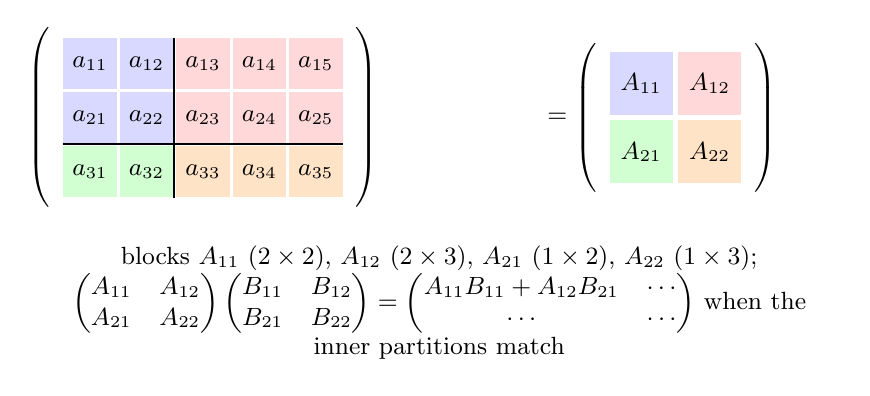
\begin{tikzpicture}[every node/.style={font=\small}]
	\matrix (M) [matrix of math nodes, nodes={minimum size=6.5mm, anchor=center}, left delimiter=(, right delimiter=), column sep=1pt, row sep=1pt] at (0,0) {
		|[fill=blue!15]| a_{11} & |[fill=blue!15]| a_{12} & |[fill=red!15]| a_{13} & |[fill=red!15]| a_{14} & |[fill=red!15]| a_{15} \\
		|[fill=blue!15]| a_{21} & |[fill=blue!15]| a_{22} & |[fill=red!15]| a_{23} & |[fill=red!15]| a_{24} & |[fill=red!15]| a_{25} \\
		|[fill=green!18]| a_{31} & |[fill=green!18]| a_{32} & |[fill=orange!22]| a_{33} & |[fill=orange!22]| a_{34} & |[fill=orange!22]| a_{35} \\
	};
	\draw[thick] (M-1-2.north east) -- (M-3-2.south east);
	\draw[thick] (M-2-1.south west) -- (M-2-5.south east);
	\node at (4.5,0) {$=$};
	\matrix (B) [matrix of math nodes, nodes={minimum size=8mm, anchor=center}, left delimiter=(, right delimiter=), column sep=2pt, row sep=2pt] at (6.0,0) {
		|[fill=blue!15]| A_{11} & |[fill=red!15]| A_{12} \\
		|[fill=green!18]| A_{21} & |[fill=orange!22]| A_{22} \\
	};
	\node[anchor=north, align=flush center, text width=10cm] at (3.0,-1.5) {blocks $A_{11}$ ($2\times2$), $A_{12}$ ($2\times3$), $A_{21}$ ($1\times2$), $A_{22}$ ($1\times3$); $\begin{pmatrix}A_{11}&A_{12}\\A_{21}&A_{22}\end{pmatrix}\begin{pmatrix}B_{11}&B_{12}\\B_{21}&B_{22}\end{pmatrix}=\begin{pmatrix}A_{11}B_{11}+A_{12}B_{21}&\cdots\\ \cdots&\cdots\end{pmatrix}$ when the inner partitions match};
\end{tikzpicture}
\end{document}
